\subsection*{1.1}
  % Implement  the  common-source  MOS  amplifier  shown  below.  
  The circuit in figure 1 was implemented in NI Multisim.\\

    \begin{figure}[h!]
        \centering
        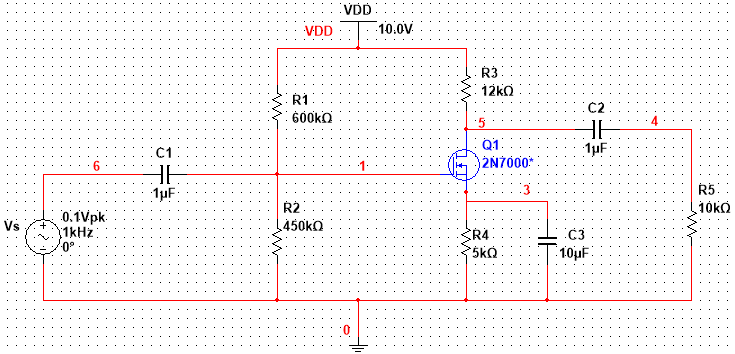
\includegraphics[width=8cm]{fig1-1-multisim.png}
        \captionof{figure}{The CS MOS amplifier implemented in Task 1.1}
    \end{figure} 

  The  transistor  model was modified to look as follows:\\
  Cgs  2 3 20E-12\\ 
  Cgd 1 2 10E-12\\
  M1 1 2 3 3 MOST1 W=500u L=2u\\
  .MODEL MOST1 NMOS(Level=3 Kp=20u W=500u L=2u Rs=20m Vto=2 Rd=1.186)\\\\

  The following parameters were used: kn =  20  $\mu$A/V2,  W/L =  250,  VT =  2  V,  Cgs =  20  pF, Cgd = 10 pF\\
\pagebreak
\subsection*{1.2}
  % Using  the  above  parameters  (here:  kn =  20  µA/V2,  W/L =  250,  VT =  2  V,  Cgs =  20  pF,
  % Cgd = 10 pF) perform the theoretical analysis of the circuit to find the voltage gain, input
  % resistance, output resistance, as well as to estimate the lower and upper 3dB frequencies.

  A theoretical analysis of the circuit in figure 1 was performed to find the voltage gain, input resistance, output resistance, as well as to estimate the lower and upper 3dB frequencies.\\\\

  To find the voltage gain the DC current, I$_D$, was found to be 379$\mu$A and used to calculate\\ g$_m$ = $\frac{1}{513.5 \Omega}$. Using the small signal t-model the midband gain was found to be $$\frac{v_o}{v_i} = |-10.615| \frac{V}{V} = 20.518 dB$$.\\\\

  The lower and upper 3dB frequencies were found doing a low and high frequency analysis of the circuit. Capacitors C$_1$1, C$_2$ and C$_3$ are much larger than capacitors C$_{gs}$ and C$_{gd}$ so for the low frequency analysis C$_{gs}$ and C$_{gd}$ can be neglected and vice versa.\\

  Calculations from the high frequency analysis using a small signal hybrid-pi model show that $$f_{H 3dB} = 2.918MHz$$

  Calculations from the low frequency analysis using a small signal T model show that $$f_{L 3dB} = 34.18Hz$$

  The input resistance of the circuit, R$_{in}$, is the parallell connection of R$_{G1}$ and R$_{G2}$, $$R_{in} = R_{G1}||R_{G2} = 257k\Omega$$
  The output resitance of the circuti, R$_{out}$, is the drain resistance, R$_D$ = 12k$\Omega$.\\\\

  All calculations can be seen in Appendix 1.\\
\pagebreak
\subsection*{1.3}
  % Determine the values of the same parameters by simulation. Note that in order to obtain
  % some  of  the  parameters  certain  changes  in  the  circuit  diagram  and/or  introducing  some
  % auxiliary elements may be necessary. 

  A simulation was done for the circuit in figure 1 to find the voltage gain, input resistance, output resistance, as well as to estimate the lower and upper 3dB frequencies.\\\\

  The drain current was found using a DC operating point analysis and the results show that \\I$_D$ = 379.244$\mu$A as seen in figure 2. The voltage at the top node is positive so the current is flowing downward from the perspective of figure 1.\\

  \begin{figure}[h!]
        \centering
        \includegraphics[width=10cm]{fig1-3-current.png}
        \captionof{figure}{DC operating point analysis used to find the drain current}
  \end{figure}

\pagebreak

  An AC analysis was used to find the gain, $$f_{L 3dB}$$ $$f_{H 3dB}$$ From the results of this analysis seen in figure 3 and 4, the gain is $$A_1 = \frac{v_o}{v_i} = 20.521 dB = 10.618 \frac{V}{V}$$ $$f_{L 3dB} = 35.592 Hz$$ $$f_{H 3dB} = 2.953MHz$$

  \begin{figure}[h!]
        \centering
        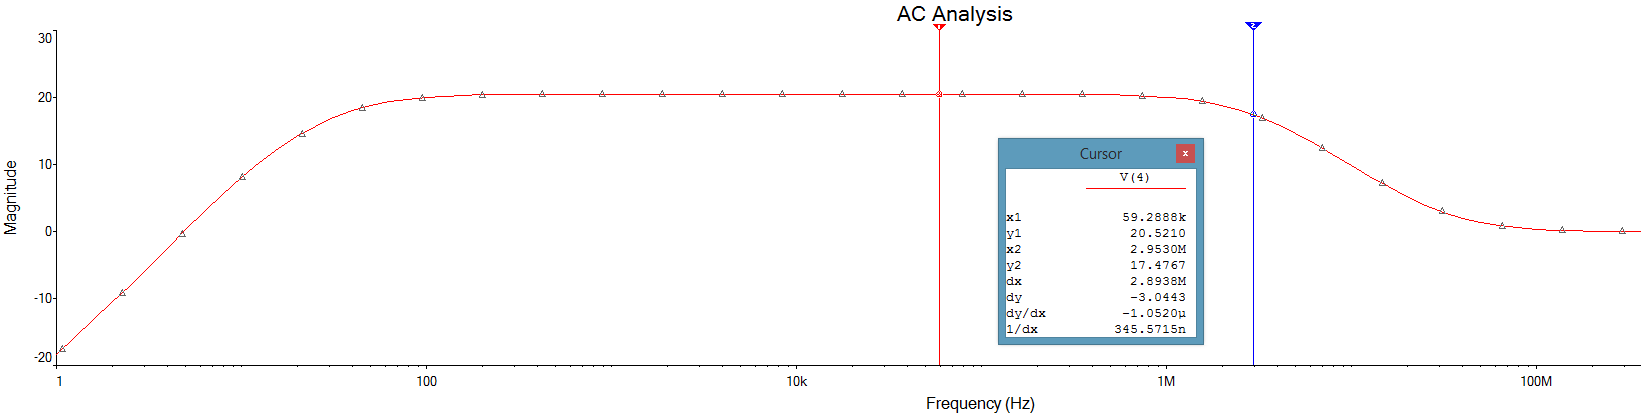
\includegraphics[width=14cm]{fig1-3-fh.png}
        \captionof{figure}{The AC analysis used to find the gain and f$_{H 3dB}$}
  \end{figure}

  \begin{figure}[h!]
        \centering
        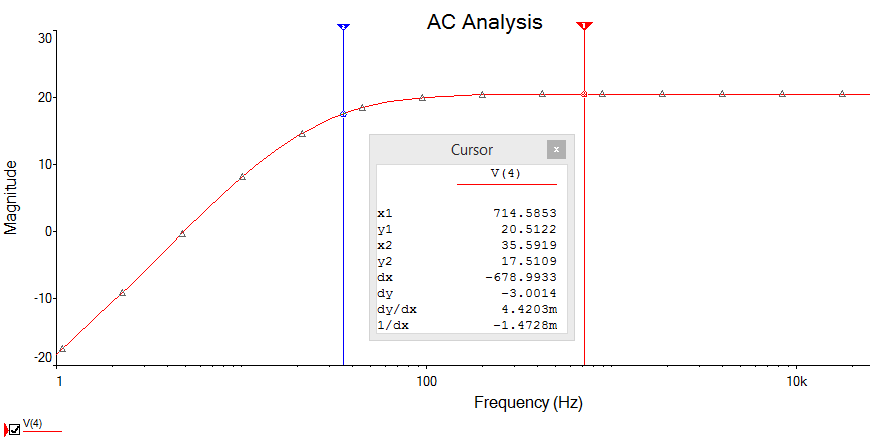
\includegraphics[width=12cm]{fig1-3-fl.png}
        \captionof{figure}{The AC analysis used to find f$_{L 3dB}$}
  \end{figure}

  \pagebreak

  The input resistance, R$_in$, was found by adding an signal resistance. The signal resistance is chosen close to what is assumed to be the correct input resistance calculated by theory in task 1.2 R$_{in}$ = $R_{G1}||R_{G2}$ = 257k$\Omega$. Using this resistance as seen in figure 5, an AC analysis seen in figure 6 is performed to see how the gain changes.\\
  
  \begin{figure}[h!]
        \centering
        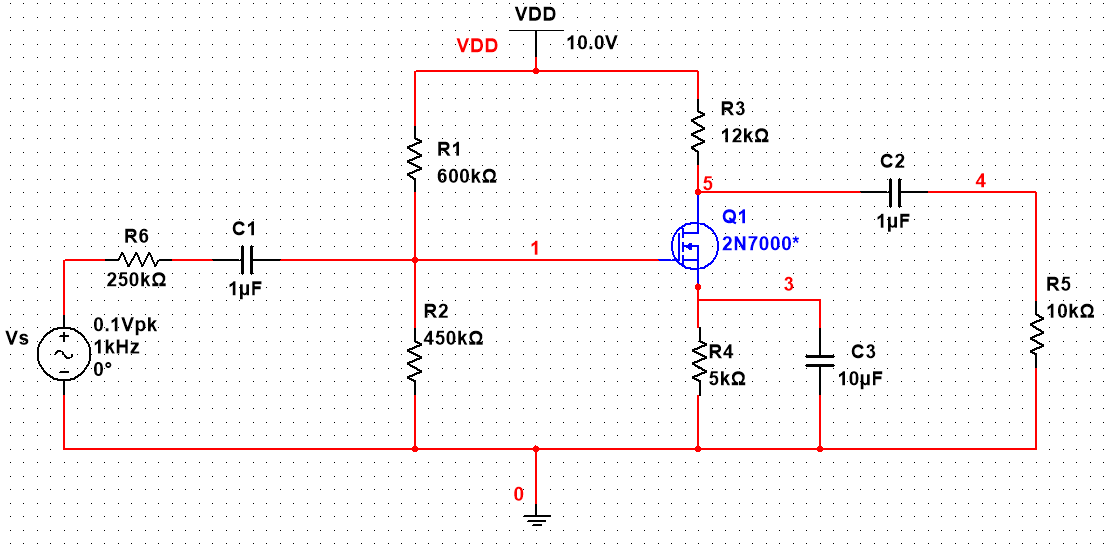
\includegraphics[width=10cm]{fig1-3-R-in-multisim.png}
        \captionof{figure}{The circuit with added signal resistance.}
  \end{figure}

  \begin{figure}[h!]
        \centering
        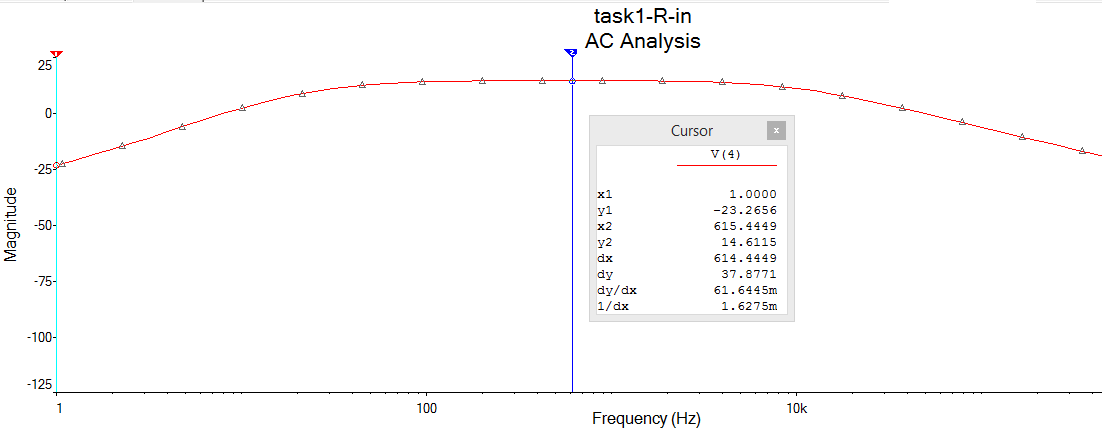
\includegraphics[width=10cm]{fig1-3-R-in.png}
        \captionof{figure}{The AC analysis used to find the new gain with input resistance.}
  \end{figure}

The gain with the added resistance is $$A_2 = 10^{14.6115/20} = 5.377 dB$$
The input resitance can then be calculated using the following formula:
$$R_{in} = \frac{R_s}{A_1 / A_2 - A_2} = \frac{R_s \cdot A_2}{A_1 - A_2} = \frac{250k\Omega \cdot 5.377}{10.618 - 5.377} = 256.5 k\Omega$$

\pagebreak

The output resitance, R$_{out}$, was found by removing the load resistance, see figure 7, from the original circuit and performing an AC analysis to see how the gain changes.\\

\begin{figure}[h!]
        \centering
        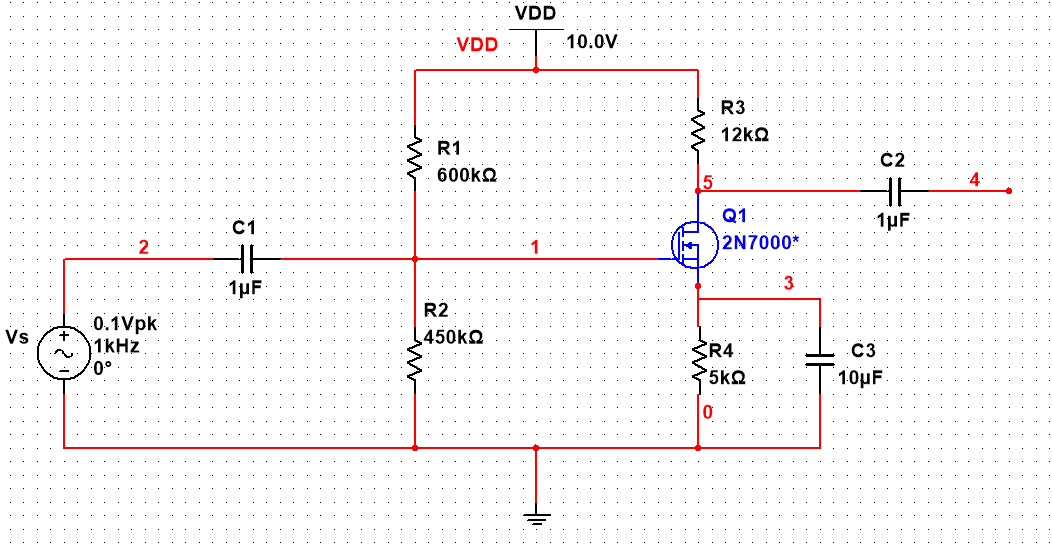
\includegraphics[width=14cm]{fig1-3-R-out-multisim.png}
        \captionof{figure}{The circuit with added signal resistance.}
  \end{figure}

  \begin{figure}[h!]
        \centering
        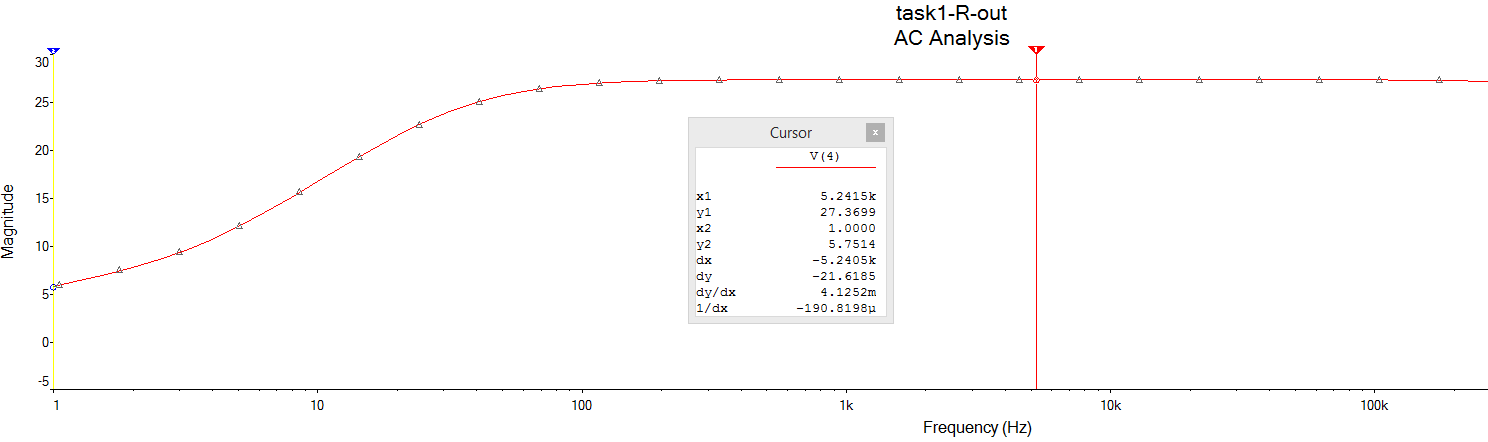
\includegraphics[width=14cm]{fig1-3-R-out.png}
        \captionof{figure}{The AC analysis used to find the new gain with input resistance.}
  \end{figure}

Obesrving the gain in figure 8 to be $$A_3 = 10^{27.3699/20} dB = 23.361 dB$$
The output resistance can then be calculated using the following formula: 
$$R_{out} = R_L\frac{A_3 - A_1}{A_1} = 10k\Omega \frac{23.361-10.618}{10.618} = 12 k\Omega$$

\pagebreak
\subsection*{1.4}
  % Compare the parameters obtained by simulation with those obtained from the theory and
  % comment upon possible differences.

  Comparison of the parameters obtained by simulation and thoes obtained from theary can be seen in the table below.\\

  \begin{table}[htbp]
     \centering
       \begin{tabular}{ c | c | c }
        \hline
         Circuit Parameters     &   Theory                  & Simulation \\
       \hline
        I$_D$                   &   379$\mu$A               &   379.244$\mu$A\\
        Midband voltage gain    &   10.615 $\frac{V}{V}$    &   10.618$\frac{V}{V}$\\
        Lower 3dB frequency     &   34.18 Hz                &   35.592 Hz\\
        Higher 3dB frequency    &   2.918 MHz               &   2.953 MHz\\
        Input Resistance        &   257 k$\Omega$           &   256.5 k$\Omega$\\
        Output Resistance       &   12 k$\Omega$            &   12 k$\Omega$\\
       \end{tabular}%
     \caption{Theory compared to simulation.}
     \label{tab:addlabel}%
    \end{table}%
  
  All measured parameters agree with parameters calculated by theory.